\documentclass[tikz,border=2pt]{standalone}
\usepackage[T1]{fontenc}
\usepackage{lmodern}
\usepackage{amsmath}
\usepackage[table]{xcolor}
\usepackage{tikz}
\usetikzlibrary{arrows.meta,calc,positioning}

\definecolor{paletteGreen}{HTML}{2A6F62}
\definecolor{paletteOrange}{HTML}{D96C3D}
\definecolor{darkblue}{RGB}{30,60,120}

\begin{document}
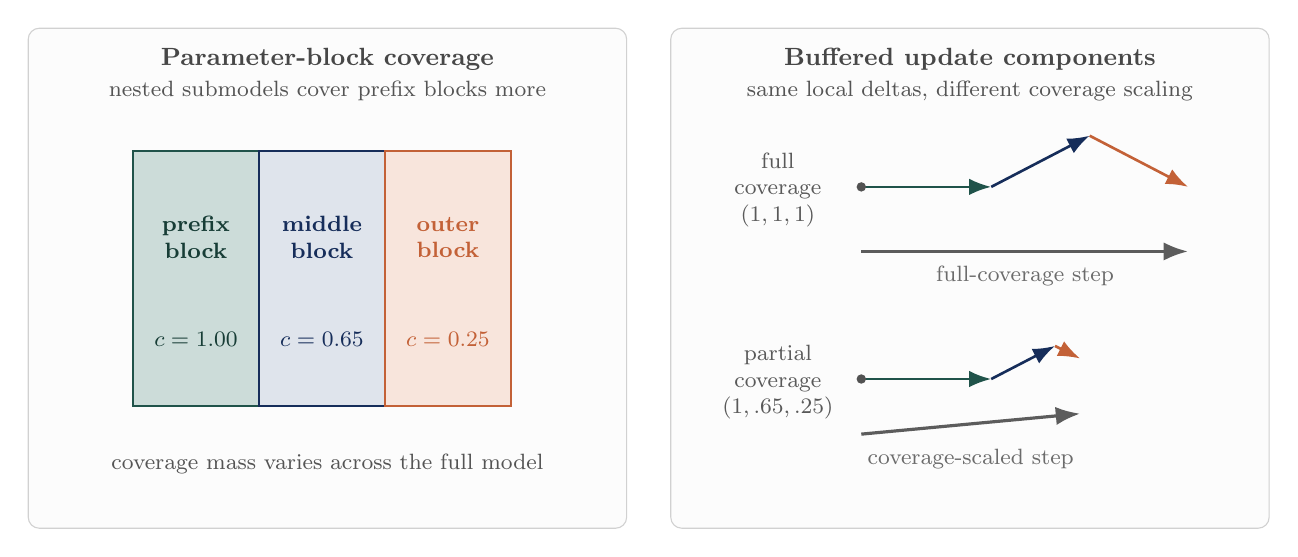
\begin{tikzpicture}[
  >=Latex,
  font=\small,
  panel/.style={draw=black!18, fill=gray!2, rounded corners=4pt, minimum width=7.60cm, minimum height=6.35cm},
  title/.style={font=\small\bfseries, text=black!72},
  smalllabel/.style={font=\footnotesize, align=center, text=black!67},
  rowlabel/.style={font=\footnotesize, align=center, text=black!65},
  blocklabel/.style={font=\footnotesize\bfseries, align=center},
  vec/.style={-{Latex[length=2.8mm]}, line width=0.95pt},
  resultant/.style={-{Latex[length=3.1mm]}, line width=1.15pt}
]
\node[panel] at (-4.08,0) {};
\node[panel] at (4.08,0) {};

\node[title] at (-4.08,2.78) {Parameter-block coverage};
\node[smalllabel] at (-4.08,2.38) {nested submodels cover prefix blocks more};

\draw[draw=black!45, line width=0.65pt] (-6.55,-1.62) rectangle (-1.75,1.62);
\draw[draw=paletteGreen!75!black, fill=paletteGreen!24, line width=0.65pt] (-6.55,-1.62) rectangle (-4.95,1.62);
\draw[draw=darkblue!75!black, fill=darkblue!14, line width=0.65pt] (-4.95,-1.62) rectangle (-3.35,1.62);
\draw[draw=paletteOrange!90!black, fill=paletteOrange!18, line width=0.65pt] (-3.35,-1.62) rectangle (-1.75,1.62);

\node[blocklabel, text=paletteGreen!55!black] at (-5.75,0.52) {prefix\\block};
\node[blocklabel, text=darkblue!75!black] at (-4.15,0.52) {middle\\block};
\node[blocklabel, text=paletteOrange!90!black] at (-2.55,0.52) {outer\\block};
\node[smalllabel, text=paletteGreen!55!black] at (-5.75,-0.78) {\(c=1.00\)};
\node[smalllabel, text=darkblue!75!black] at (-4.15,-0.78) {\(c=0.65\)};
\node[smalllabel, text=paletteOrange!90!black] at (-2.55,-0.78) {\(c=0.25\)};
\node[smalllabel] at (-4.08,-2.36) {coverage mass varies across the full model};

\node[title] at (4.08,2.78) {Buffered update components};
\node[smalllabel] at (4.08,2.38) {same local deltas, different coverage scaling};

\node[rowlabel] at (1.64,1.12) {full\\coverage\\\((1,1,1)\)};
\coordinate (eq0) at (2.70,1.16);
\coordinate (eq1) at (4.35,1.16);
\coordinate (eq2) at (5.60,1.81);
\coordinate (eq3) at (6.85,1.16);
\draw[vec, draw=paletteGreen!75!black] (eq0) -- (eq1);
\draw[vec, draw=darkblue!75!black] (eq1) -- (eq2);
\draw[vec, draw=paletteOrange!90!black] (eq2) -- (eq3);
\fill[black!68] (eq0) circle (1.7pt);
\draw[resultant, draw=black!64] (2.70,0.34) -- (6.85,0.34);
\node[smalllabel, text=black!58] at (4.78,0.03) {full-coverage step};

\node[rowlabel] at (1.64,-1.32) {partial\\coverage\\\((1,.65,.25)\)};
\coordinate (un0) at (2.70,-1.28);
\coordinate (un1) at (4.35,-1.28);
\coordinate (un2) at (5.16,-0.86);
\coordinate (un3) at (5.48,-1.02);
\draw[vec, draw=paletteGreen!75!black] (un0) -- (un1);
\draw[vec, draw=darkblue!75!black] (un1) -- (un2);
\draw[vec, draw=paletteOrange!90!black] (un2) -- (un3);
\fill[black!68] (un0) circle (1.7pt);
\draw[resultant, draw=black!64] (2.70,-1.98) -- (5.48,-1.72);
\node[smalllabel, text=black!58] at (4.09,-2.30) {coverage-scaled step};
\end{tikzpicture}
\end{document}
